%نام و نام خانوادگی:
%شماره دانشجویی: 
\مسئله{ }

\پاسخ{
\begin{enumerate}
	\item
		\begin{latin}
			\begin{table}[H]
				\begin{tabular}{c|c}
					Instruction & Live Variables\\
					\hline
					a = b & {b, e} \\
					c = 7 + 7 * e & {a, b, e}\\
					d = a & {a, b, c}\\
					a = d * d & {b, c, d}\\
					d = 5 * a & {a, b, c}\\
					f = c * 5 + 10 & {b, c, d}\\
					f = d - f & {b, d, f}\\
					c = f + 1  & {b, f}\\
					e = c * b  & {b, c}\\
							& {b, c}\\
				\end{tabular} 
			\end{table} 
		\end{latin}
باتوجه به جدول بالا، گراف تداخل رجیسترها به شکل زیر خواهد بود:
		\newline
		\begin{figure}[H]
			\centering
			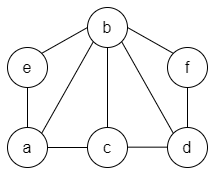
\includegraphics[width=\linewidth / 2]{./commons/Q8_1.png}
			\label{fig:Q8}
		\end{figure}
	\item
با توجه به این که در گراف، دور به طول 3 داریم، در بهترین حالت سه رجیستر نیاز است. سه عدد رجیستر را امتحان میکنیم تا ببینیم کفایت می‌کند یا خیر. که خواهیم دید کفایت می‌کند.
		\newline
ابتدا e را برمیداریم. سپس a را برمیداریم. بعد c و بعد d را برمیداریم. تا اینجا، هر راسی را که برداشتیم، دو عدد یال خروجی داشت. حال f و در آخر b را برمیداریم. 
		\newline
حال شروع به رنگ کردن می‌کنیم. ابتدا b را میاوریم و آبی میکنیم. سپس f را قرمز میکنیم و بعد آن، d را سبز. بعدی نوبت c است. آن را قرمز میکنیم. بعدی a است و سبز میشود. و آخری که e خواهدبود، قرمز میگردد.
		\newline
تصویر پایین، نتیجه پایانی را نشان میدهد:
		\newline
		\begin{figure}[H]
			\centering
			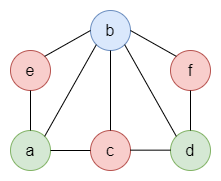
\includegraphics[width=\linewidth / 2]{./commons/Q8_2.png}
			\label{fig:Q8_2}
		\end{figure}
\end{enumerate}
}

